\input{settings}
\setlength{\emergencystretch}{2em}
\titleformat{\section}
  {\small\bfseries\raggedright}
  {}{0em}
  {}
  [{\color{WHU_Blue}\titlerule}]
\titlespacing*{\section}{0cm}{0.85em}{0.60em}
\titlespacing*{\subsection}{0cm}{0.50em}{0.30em}
\setlist[itemize]{topsep=0.20em, itemsep=0.20em, parsep=0em, partopsep=0em, leftmargin=1.25em}
\setlist[enumerate]{topsep=0.20em, itemsep=0.20em, parsep=0em, partopsep=0em, leftmargin=1.35em}
\renewcommand{\arraystretch}{0.98}
\renewcommand{\CJKglue}{\hskip 0.018em}

% 个人信息
%  cd C:\Users\31087\Documents\Obsidian_Vault\Resume\template
%  xelatex main_perception.tex
\newcommand{\school}{江南大学 · 控制科学与工程}

\newcommand{\resumeDecor}{
    \begin{tikzpicture}[remember picture, overlay]
        \node[anchor=north, inner sep=0pt](header) at (current page.north){
            
\includegraphics[width=\paperwidth]{images/header.png}
        };
        \node[anchor=west](school_logo) at (header.west){
            \hspace{0.5cm}
            
\includegraphics[width=0.15\textwidth]{images/whu_logo_1.png}
        };
        \node[anchor=east](school_name) at(header.east){
            \textcolor{white}{\textbf{\school}}
            \hspace{0.5cm}
        };
    \end{tikzpicture}

    \begin{tikzpicture}[remember picture, overlay]
        \node[opacity=0.05] at(current page.center){
            
\includegraphics[width=0.68\paperwidth, keepaspectratio]{images/whu_logo_big.png}
        };
    \end{tikzpicture}
}

\newcommand{\sectionIcon}[2]{\makebox[\widthof{#1}][c]{\color{WHU_Blue}{#1}}\quad #2}

%%%%%%%%%%%%%%%%%%%%
% 简历正文
%%%%%%%%%%%%%%%%%%%%
\begin{document}
\resumeDecor
\vspace*{-3.15em}
\scriptsize
\linespread{1.10}\selectfont

% 个人信息
\begin{minipage}{0.80\textwidth}
    \section[个人信息]{\sectionIcon{\faAddressCard}{个人信息}}
    \footnotesize
    \begin{tabularx}{\linewidth}{p{\widthof{求职意向:}}Xp{\widthof{最高学历:}}X}
        姓\ \ \ \ \ \ \ \ 名: & 梁邦一 &
        性\ \ \ \ \ \ \ \ 别: & 男 \\
        邮\ \ \ \ \ \ \ \ 箱: & yuejinai55@gmail.com &
        电\ \ \ \ \ \ \ \ 话: & +86 15515602693 \\
        英语等级: & CET-6 &
        求职意向: & 自动驾驶感知工程师 \\
    \end{tabularx}
\end{minipage}
\hfill
\begin{minipage}{0.11\textwidth}
    \vspace{2.0em}
    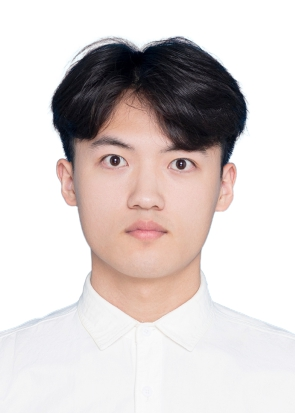
\includegraphics[width=\linewidth]{images/avatar.png}
\end{minipage}
\vspace{-0.60em}

\section[教育背景]{\sectionIcon{\faGraduationCap}{教育背景}}
\begin{itemize}
    \item {\textbf{控制科学与工程硕士，江南大学}}（\hl{中国科学院沈阳自动化研究所 · 机器人与智能系统全国重点实验室联合培养}） \hfill {2024.06--2027.06}
    \item {\textbf{自动化学士，郑州轻工业大学}} \hfill {2020.09--2024.06}
\end{itemize}

% 实习经历
\section[实习经历]{\sectionIcon{\faBriefcase}{实习经历}}
{\small\textbf{CARIZON（大众×地平线合资智驾）}}\quad 感知数据部门算法实习生 \hfill {2026.06--至今}\\
{\scriptsize\color{WHU_Blue} 道路视觉感知与长尾挖掘 / VLM 后训练 / 感知数据闭环}
\begin{itemize}
    \item \textbf{长尾场景视觉挖掘：}面向红绿灯、交通标识、车辆、行人、锥桶等道路长尾目标，搭建 Grounding DINO 目标定位 + Qwen3-VL 细粒度属性判别 + 视觉 Embedding 检索的组合挖掘链路；主导设计并落地“以图搜图 2.0”（相似性 + 正负例精排做场景召回与标签生产，不依赖检测 / 分割等额外模型），累计交付 \hl{50+ 感知标签}，单标签样本 >1.5 万、\hl{整体标签准确率超 80\%}。
    \item \textbf{场景 Tagger 挖掘：}融合车载多路传感器与回灌数据设计规则化挖掘算子，红绿灯自车转向 Tagger 在 \hl{3 万条路口数据}中筛选约 3000 条转向 Clip，\hl{标签验收准确率达 90\%、挖掘召回提升 10\%}，直接支撑感知模型训练与标签库建设。
    \item \textbf{VLM 细粒度识别 SFT：}围绕闸机杆 / 限高杆五分类任务，完成数据清洗、标注校验与 Prompt 迭代，在 LLaMA-Factory 上完成 \hl{13 轮 SFT 实验迭代}（LoRA $\rightarrow$ 全参、高分辨率图像、手写 CoT 混合双 prompt），在 \hl{4 机 8 卡 H20 集群}完成全参数 SFT，\hl{测试集准确率 0.8984 创历史新高}；并在 GT 生产平台落地 CoT 标注工具链，形成“人工标注 $\rightarrow$ SFT 训练数据”闭环。
\end{itemize}

\vspace{0.30em}
{\small\textbf{优奇智能科技有限公司（优必选子公司）}}\quad 人形机器人感知算法实习生 \hfill {2026.02--2026.05} \\
{\scriptsize\color{WHU_Blue} Jetson AGX Orin 端侧部署 / TensorRT 推理加速 / 目标检测与实例分割}
\begin{itemize}
    \item \textbf{Jetson AGX Orin 端侧部署与推理加速：}负责 R11 接待机器人视觉感知模型在 NVIDIA Jetson AGX Orin 端侧计算平台的部署，围绕 TensorRT 推理引擎完成 PyTorch $\rightarrow$ ONNX $\rightarrow$ TensorRT 模型转换、量化与算子性能优化，\hl{推理延迟降低 20\%}，在真机跑通目标检测与实例分割实时推理链路，形成\hl{“训练—部署—实机验证”端到端工程闭环}。
    \item \textbf{检测与分割模型训练：}完成 YOLO11s-seg 数据配置、模型训练、参数调优与效果验证，并针对复杂光照、视角变化与局部遮挡等条件定位识别表现问题，建立\hl{可复用的目标检测与实例分割训练流程}。
    \item \textbf{Bad Case 数据闭环：}负责多场景视觉数据清洗、类别一致性检查与标注质检；针对误检、漏检及分割边界异常样本，从数据覆盖、标注质量、模型能力等维度归因并制定定向补数方案，形成\hl{“模型评估 $\rightarrow$ Bad Case 归因 $\rightarrow$ 数据改进”的迭代闭环}。
\end{itemize}

\vspace{0.04em}
\section[科研与项目经历]{\sectionIcon{\faFlask}{科研与项目经历}}
{\small\textbf{面向具身智能灵巧操作的肌电-力融合感知与灵巧手抓取控制系统（灵心巧手） · 负责人}} \hfill {2025.02--2026.02} \\
{\scriptsize\color{WHU_Blue} 多传感器融合 / Transformer 与 Conformer 时序建模 / ROS2 与 MuJoCo 仿真}
\begin{itemize}
    \item \textbf{多模态感知系统：}面向 Linker Hand G20 灵巧手，搭建视觉、sEMG、力 / 触觉及 MuJoCo 仿真的\hl{多模态融合感知系统}，完成 Delsys Trigno、Sensel 等多通道传感器高频同步采集、时间戳对齐与任务标注，形成可复现的数据入口。
    \item \textbf{时序感知建模：}基于 PyTorch 开展 Transformer / 轻量 Conformer 时序特征建模，实现肌电信号到指尖力的建模，支持\hl{力等级分类与连续力值回归双任务}；相关 sEMG-Conformer 研究在 Biomedical Signal Processing and Control 在修。
    \item \textbf{系统集成与仿真：}基于 ROS2 构建视觉—仿真策略—sEMG—触觉的模块化感知控制链路，打通 MuJoCo 仿真与真机联调，构成 \hl{Sim-to-Real 端到端方案雏形}；多传感器同步与融合链路可迁移至激光雷达 + 摄像头 + 毫米波雷达的融合感知。
\end{itemize}

\section[论文与研究成果]{\sectionIcon{\faBook}{论文与研究成果}}
\begin{itemize}
    \item \hl{已录用 · 第一作者}（JCR 一区 / 中科院二区）：Sensing Technologies for Hand Gesture Recognition in Human-Robot Interaction: A Review. IEEE Sensors Journal, 2025, 26(2): 1501-1519. 综述数据手套、视觉与肌电等手势感知技术路线及精度、侵入性与成本取舍。% 若已见刊可改为“已发表”
    \item \hl{In Revision（在修）}（JCR 一区 / 中科院二区 Top）：sEMG Conformer: Synergizing Local-Global Spatiotemporal Features for Continuous Force Estimation. Biomedical Signal Processing and Control. 卷积局部建模 + 自注意力全局建模，实现肌电的力等级分类与连续力值回归。% TODO: 补充作者排序（第一作者/共一/第几作者）
    \item \hl{Under Review（在投）}（JCR 一区 / 中科院二区）：Dexterous Hand Grasping Control Based on Multimodal Sensory Fusion and Simulation Reinforcement Learning. 基于 MuJoCo 强化学习生成抓取姿态，融合视觉、肌电与触觉构建灵巧手闭环控制系统。% TODO: 补充作者排序
\end{itemize}

% 专业技能
\section[专业技能]{\sectionIcon{\faWrench}{专业技能}}
\begin{itemize}
    \item \textbf{视觉感知：}目标检测、实例分割、开放词汇检测、细粒度属性识别、视觉 Embedding 检索；YOLO11s-seg、Grounding DINO、Qwen3-VL。
    \item \textbf{模型训练：}PyTorch、Transformer、Conformer、LLaMA-Factory（LoRA / 全参数 SFT）、Qwen3-VL-8B、多机多卡分布式训练。
    \item \textbf{端侧部署：}TensorRT、ONNX、NVIDIA Jetson AGX Orin、CUDA、模型量化与算子优化。
    \item \textbf{数据闭环：}规则 Tagger、回灌数据挖掘、标注质检、Bad Case 归因、标签库建设、训练 / 验证 / 测试集划分。
    \item \textbf{工程与仿真：}Python、C++、Linux、Git、Docker、ROS2、MuJoCo。
    \item \textbf{方向储备：}激光雷达 / 毫米波雷达多传感器融合、BEV Perception（BEVFormer / BEVFusion）、Occupancy 网络、动态目标跟踪。
\end{itemize}

% 荣誉与综合素质
\section[荣誉与综合素质]{\sectionIcon{\faStar}{荣誉与综合素质}}
\begin{itemize}
    \item 中国机器人大赛暨 RoboCup 机器人世界杯中国赛 \hl{国家三等奖}｜校一等奖学金（2025、2026）｜优秀毕业生。
    \item 本科期间曾任班长，硕士期间担任党支部书记。
\end{itemize}

\end{document}
